\documentclass[handout]{beamer}

\usepackage[frenchb]{babel}
\usepackage[T1]{fontenc}
\usepackage[utf8x]{inputenc}
 
\usetheme{Berkeley}
\usecolortheme{crane}
\useinnertheme{rounded}

\title[MecaFlux]{Présentation projet : Modélisation de l'écoulement de l'air autour d'un camion}
\author{Clément \bsc{Rousseau} \& Alexandre \bsc{Vieira}}
\institute{INSA de Rouen}
\date{20 mai 2014}


\AtBeginSection[]
{
	\begin{frame}
		\frametitle{Sommaire}
		\tableofcontents[currentsection, hideothersubsections]
	\end{frame}
}

\begin{document}

\begin{frame}
\titlepage
\end{frame}

\begin{frame}
	\frametitle{Sommaire}
	\tableofcontents
\end{frame}

\section[Maillages]{Présentation des maillages}
 
\begin{frame}
	\frametitle{Maillage n°1}
	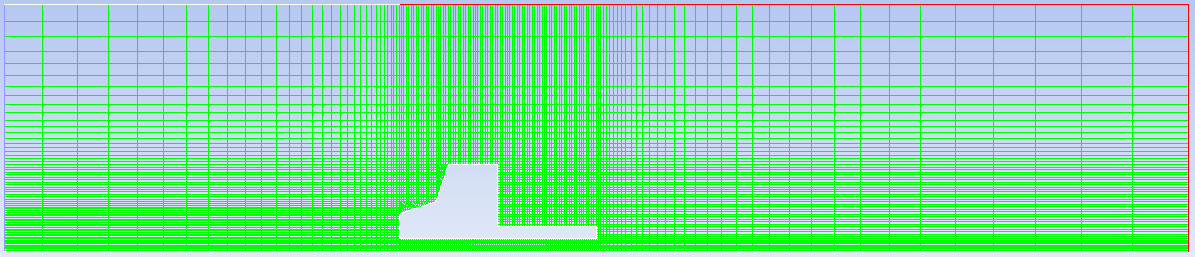
\includegraphics[scale=0.38]{../images/camion_cabine_1.png}
\end{frame}

\begin{frame}
	\frametitle{Maillage n°2}
	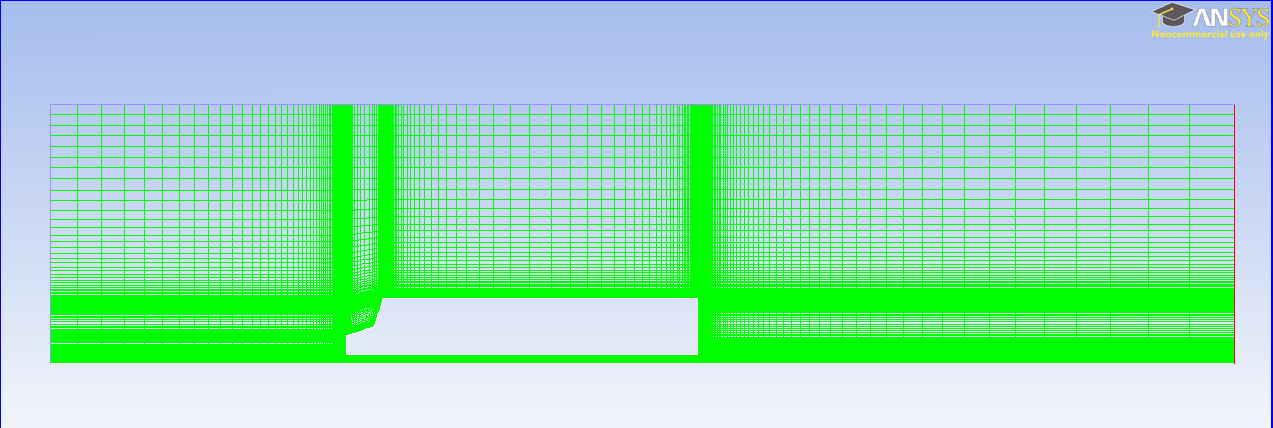
\includegraphics[scale=0.3]{../images/remorque1_mesh.png}
\end{frame}

\begin{frame}
	\frametitle{Maillage n°3}
	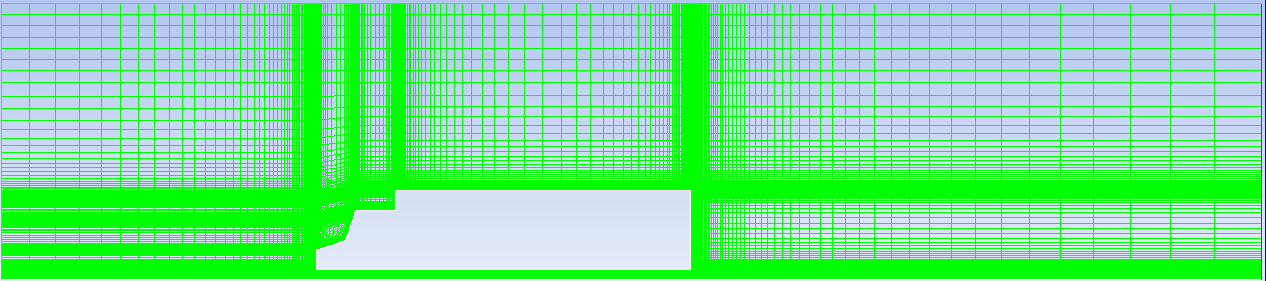
\includegraphics[scale=0.35]{../images/camion_remorque_1.png}
\end{frame}

\begin{frame}
	\frametitle{Maillage n°4}
	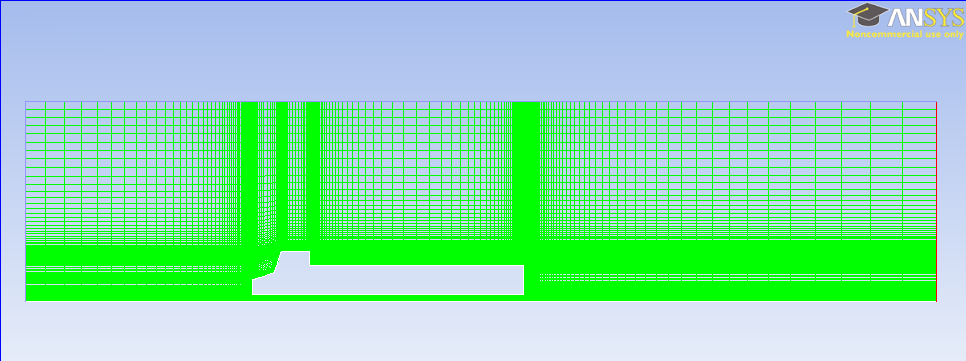
\includegraphics[scale=0.38]{../images/remorque3_mesh.png}
\end{frame}

\section[Résultats]{Analyse des résultats obtenus}
\begin{frame}
	\frametitle{Maillage n°1}
	\begin{center}
	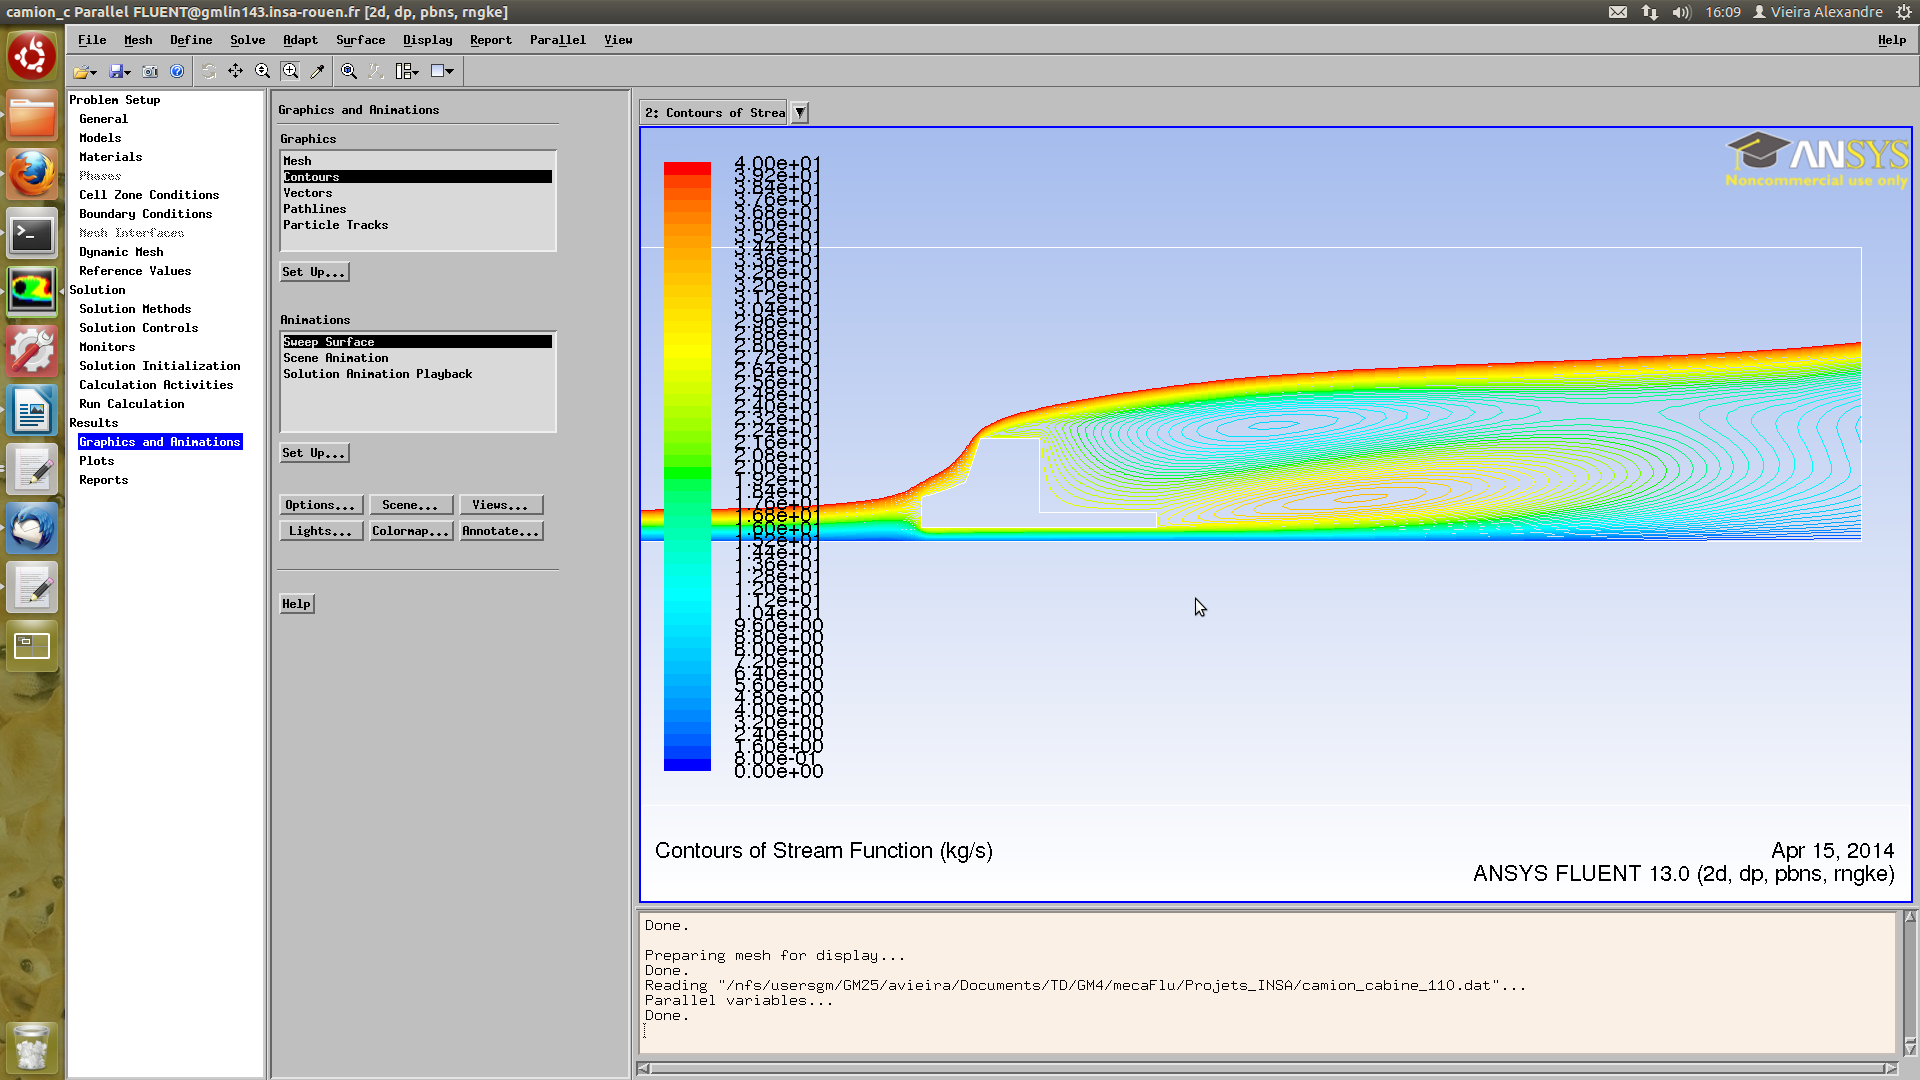
\includegraphics[scale=0.15]{../resultsCx/camion110_stream.png}\\
	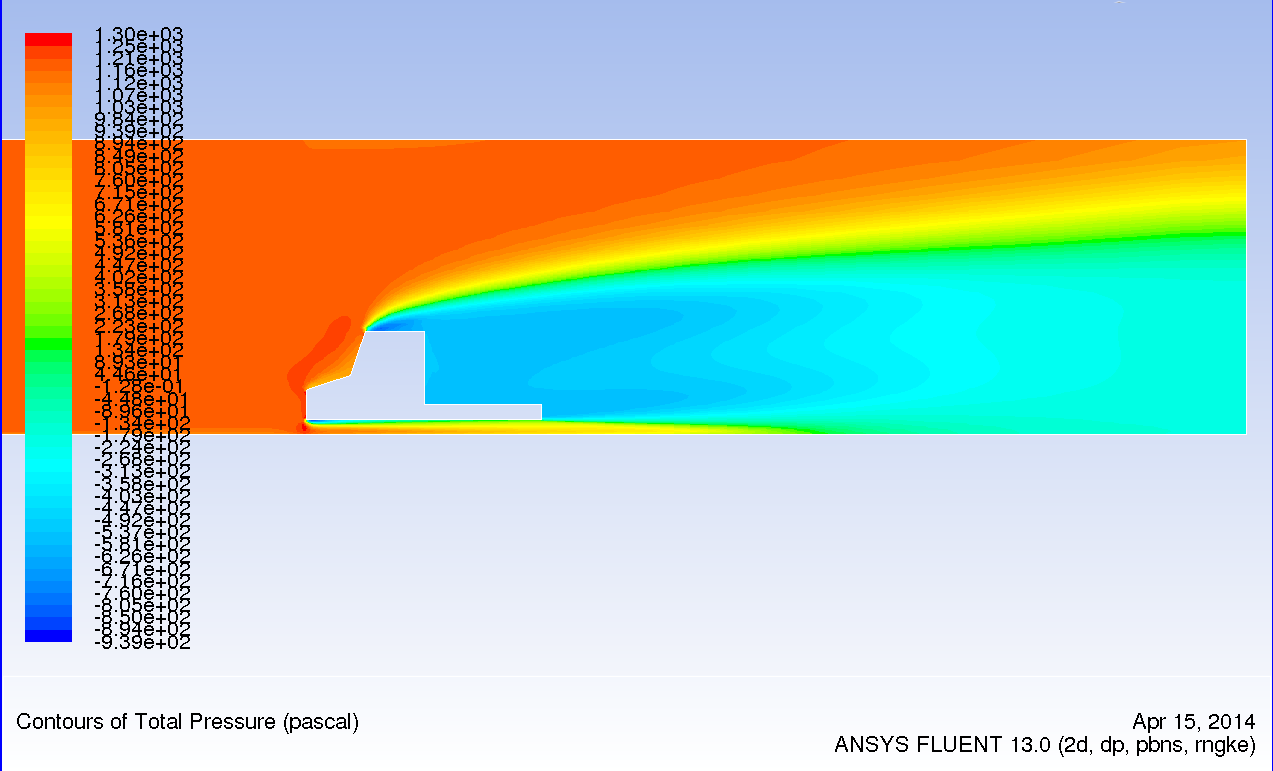
\includegraphics[scale=0.15]{../resultsCx/camion110_pressure.png}
	\end{center}
\end{frame}

\begin{frame}
	\frametitle{Maillage n°2}
	\begin{center}
	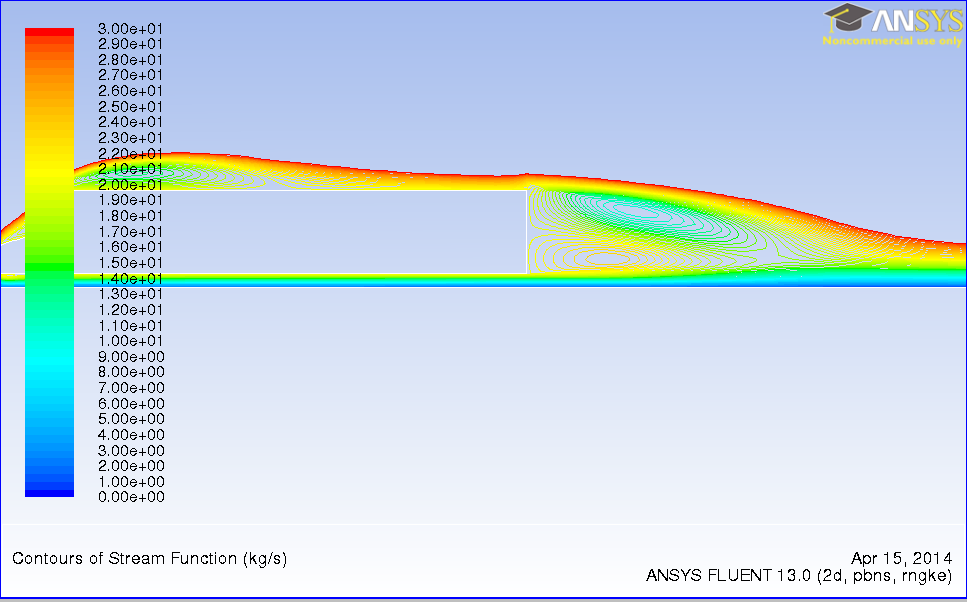
\includegraphics[scale=0.2]{../resultsCx/remorque1_110_stream.png}\\
	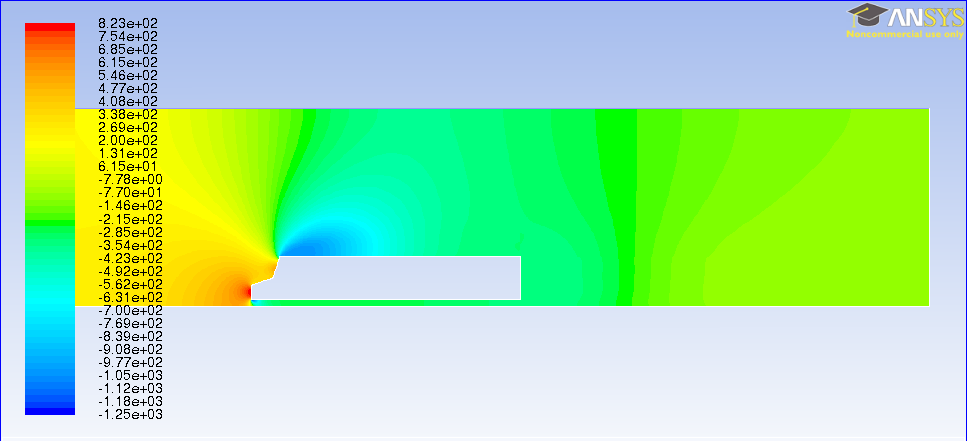
\includegraphics[scale=0.2]{../resultsCx/remorque1_110_pression.png}
	\end{center}
\end{frame}

\begin{frame}
	\frametitle{Maillage n°3}
	\begin{center}
	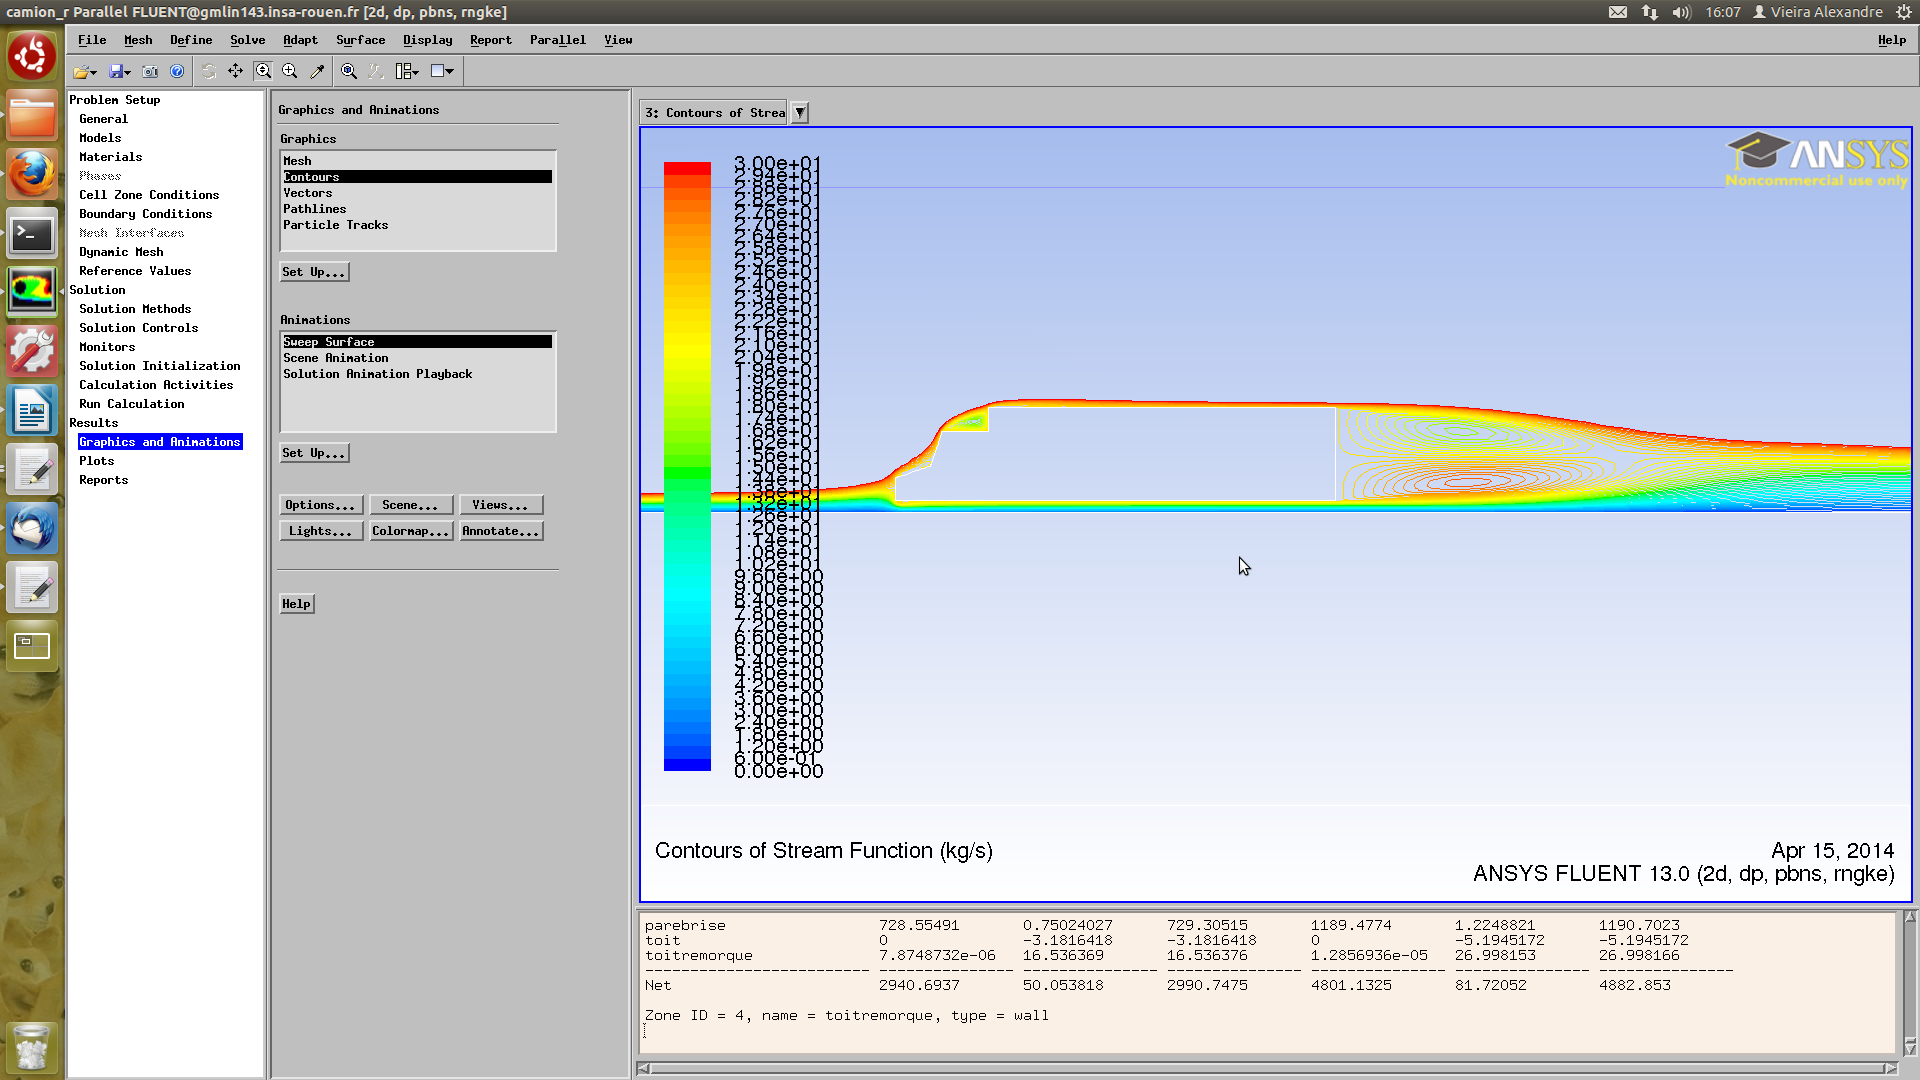
\includegraphics[scale=0.15]{../resultsCx/remorque2_110_stream.png}\\
	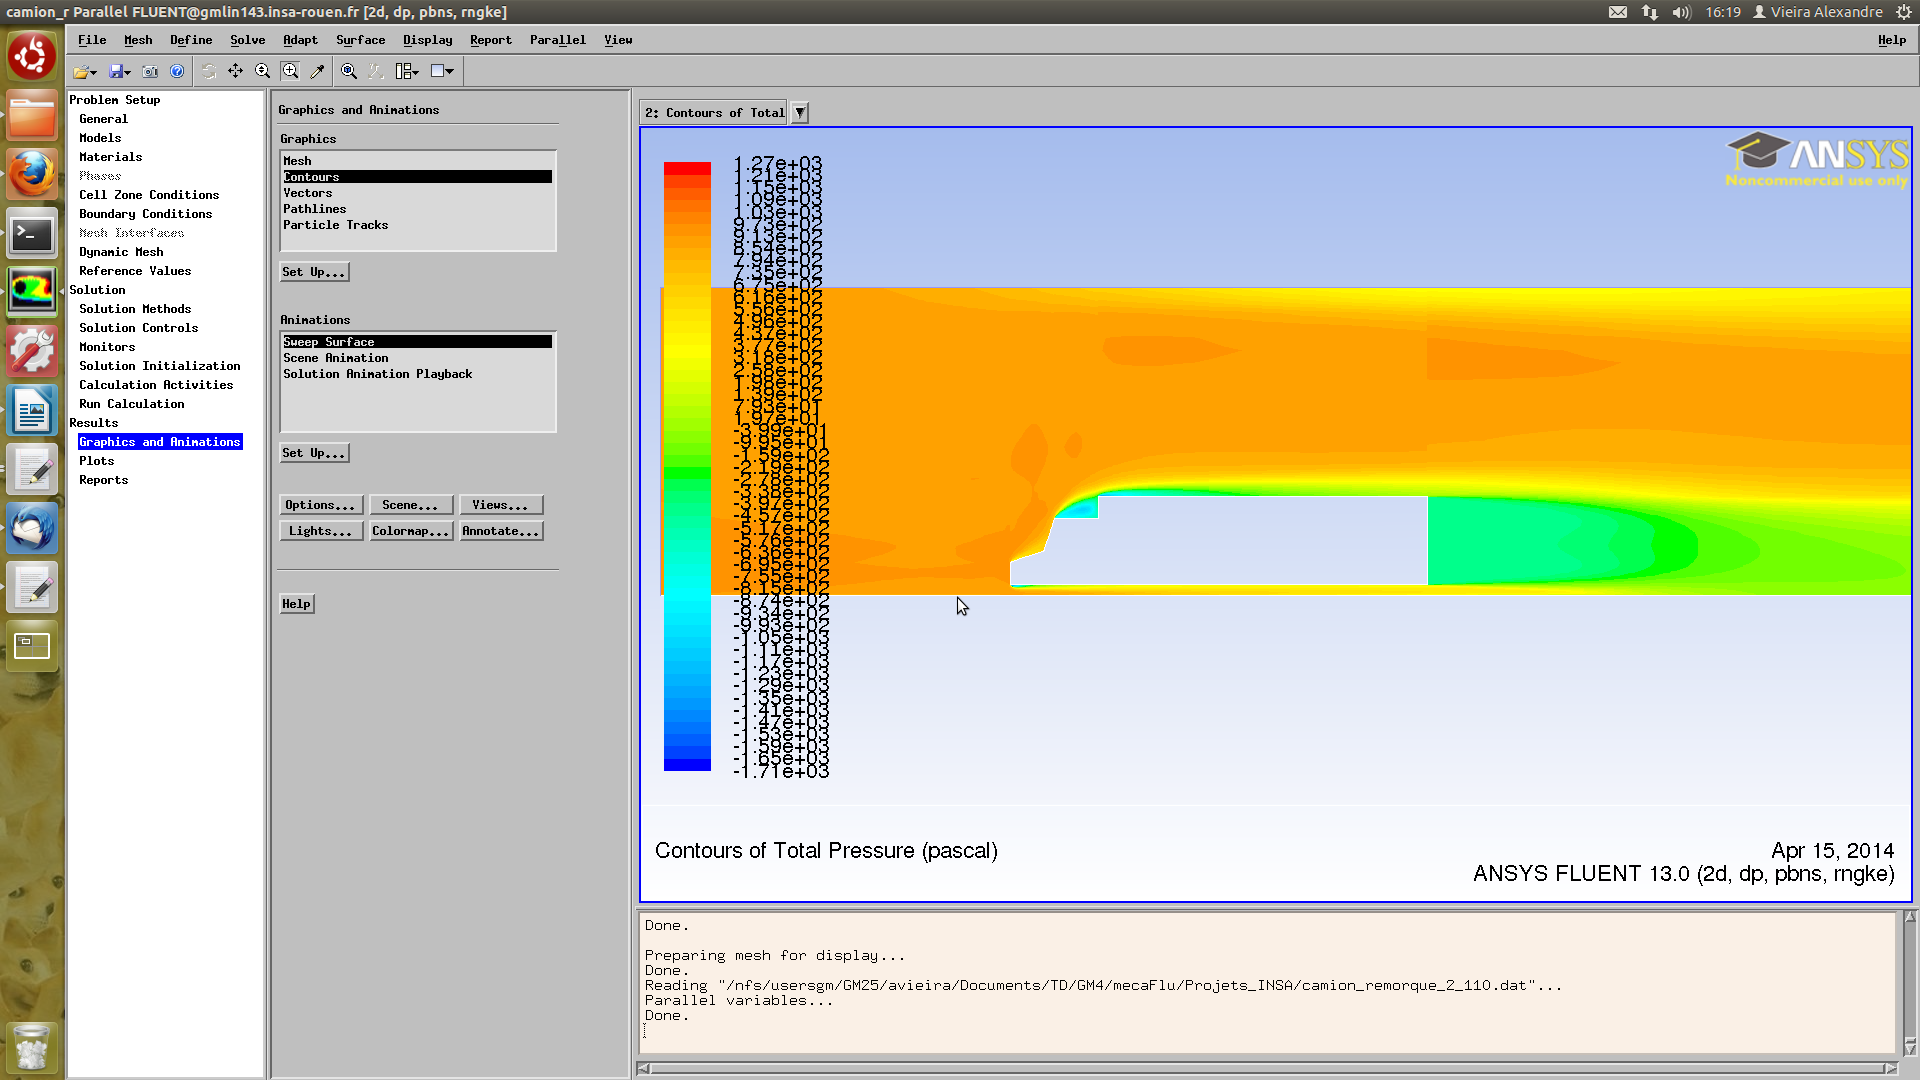
\includegraphics[scale=0.15]{../resultsCx/remorque2-110_pressure.png}
	\end{center}
\end{frame}

\begin{frame}
	\frametitle{Maillage n°4}
	\begin{center}
	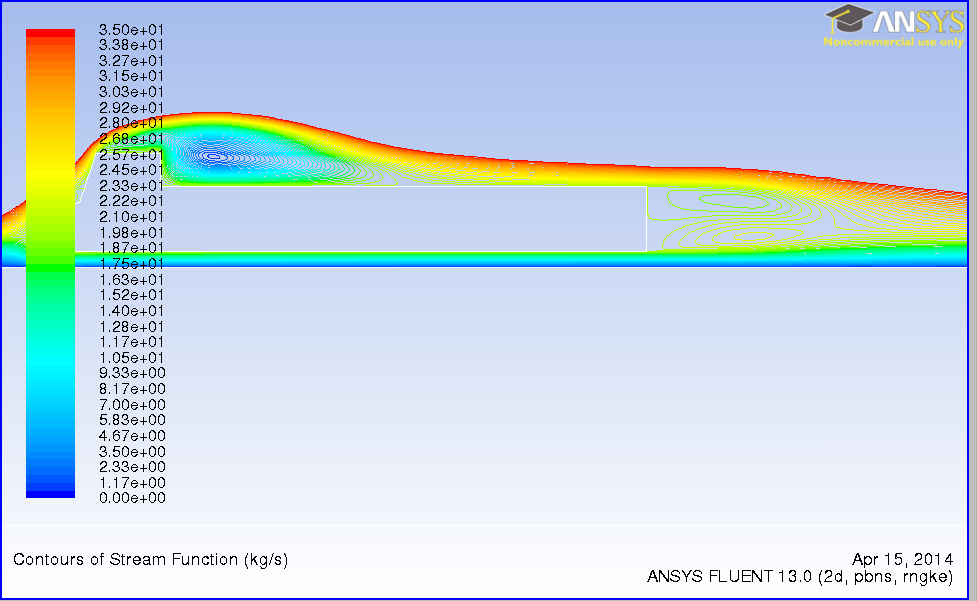
\includegraphics[scale=0.21]{../resultsCx/remorque3_110stream.png}\\
	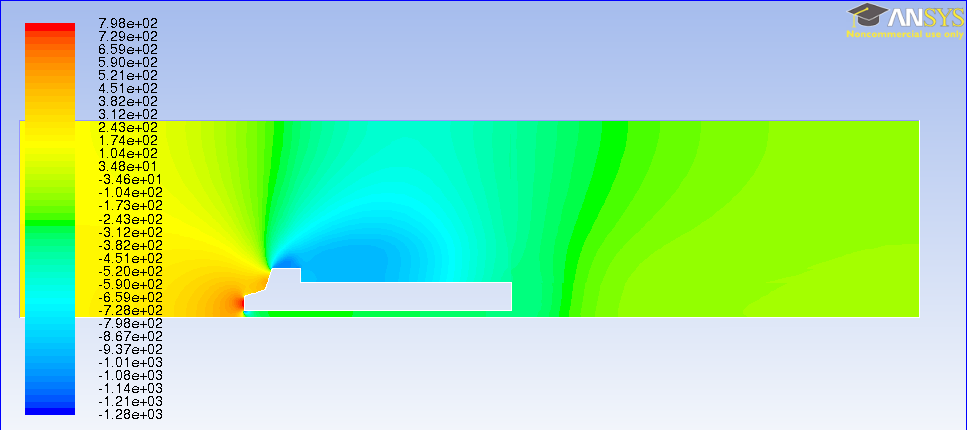
\includegraphics[scale=0.21]{../resultsCx/rem3_press_110.png}
	\end{center}
\end{frame}

\section{Commentaires}
\begin{frame}
	\frametitle{Commentaires}
	\begin{itemize}
		\item Tenue de la route
		\item Consommation
		\item Optimisation de la cargaison
	\end{itemize}
\end{frame}

\begin{frame}
	\frametitle{Commentaires}
	\begin{center}\begin{tabular}{|l|r r r|}
	\hline
	\multicolumn{4}{|c|}{Forces - Direction Vector (1 0 0)} \\
	\hline
			&   \multicolumn{3}{c|}{Forces (n)} \\
	\hline
	Zone                &     Pressure    &   Viscous     &   Total      \\
	\hline
	arriere\_cabine      &     1353.4712   &   0           &   1353.4712  \\
	arriere\_camion     &      272.26549   &   0           &   272.26549  \\ 
	capot               &     415.56441    &  1.5682516    &  417.13266   \\
	pare-brise          &     1048.325     &  0.98624219   &  1049.3113   \\
	pare-bufle          &     1121.3655    &  0            &  1121.3655   \\
	plancher            &     0            &  20.532769    &  20.532769   \\
	plateau             &     0            &  -0.50339391  &  -0.50339391 \\
	toit                &     0            &  -1.7254131   &  -1.7254131  \\
	\hline
	\hline
	Net                 &     4210.9917    &  20.858455    &  4231.8501   \\
	\hline
	\end{tabular}\end{center}
\end{frame}

\begin{frame}
	\frametitle{Commentaires}
	\begin{center}\begin{tabular}{|l|r r r|}
	\hline
	\multicolumn{4}{|c|}{Forces - Direction Vector (0 1 0)} \\
	\hline
			&   \multicolumn{3}{c|}{Forces (n)} \\
	\hline
	Zone                &     Pressure    &   Viscous     &   Total      \\
	\hline
	arriere\_cabine      &     0           &   0.24353637  &   0.24353637  \\ 
	arriere\_camion      &     0           &   -0.090688751&   -0.090688751\\ 
	capot               &     -1246.6932  &   0.52275052  &   -1246.1705  \\ 
	pare-brise          &     -349.44168  &   2.9587266   &   -346.48295  \\ 
	pare-bufle          &     0           &   -0.48552695 &   -0.48552695 \\ 
	plancher            &     -4611.9409  &   0           &   -4611.9409  \\ 
	plateau             &     2179.7929   &   0           &   2179.7929   \\ 
	toit                &     1747.0896   &   0           &   1747.0896   \\ 
	\hline
	\hline
	Net                 &     -2281.1934  &   3.1487978   &   -2278.0446  \\ 
	\hline
	\end{tabular}\end{center}
\end{frame}

\end{document}
